\documentclass[../main.tex]{subfiles}

\begin{document}

%    abandoned

    \gls{cloud_native}, design for failure/ephemeral so it can be run on k8 \ldots

    network limitations, multicast, can applications be migrated that run on dedicated hardware for ultra low latency.

    Build for failure, containers are ephemeral.
    Establish patters for \gls{cloud_native} development.
    How do applications communicate between two clusters.
    Can we create a flat network over two clusters so talking to services that are not exposed over a load balancer is possible.
    Use a service registry that keeps track of all exposed services across execution environments (Fig.~\ref{fig:deploy_svc_registry}).

    \begin{figure}[h]
        \centering
        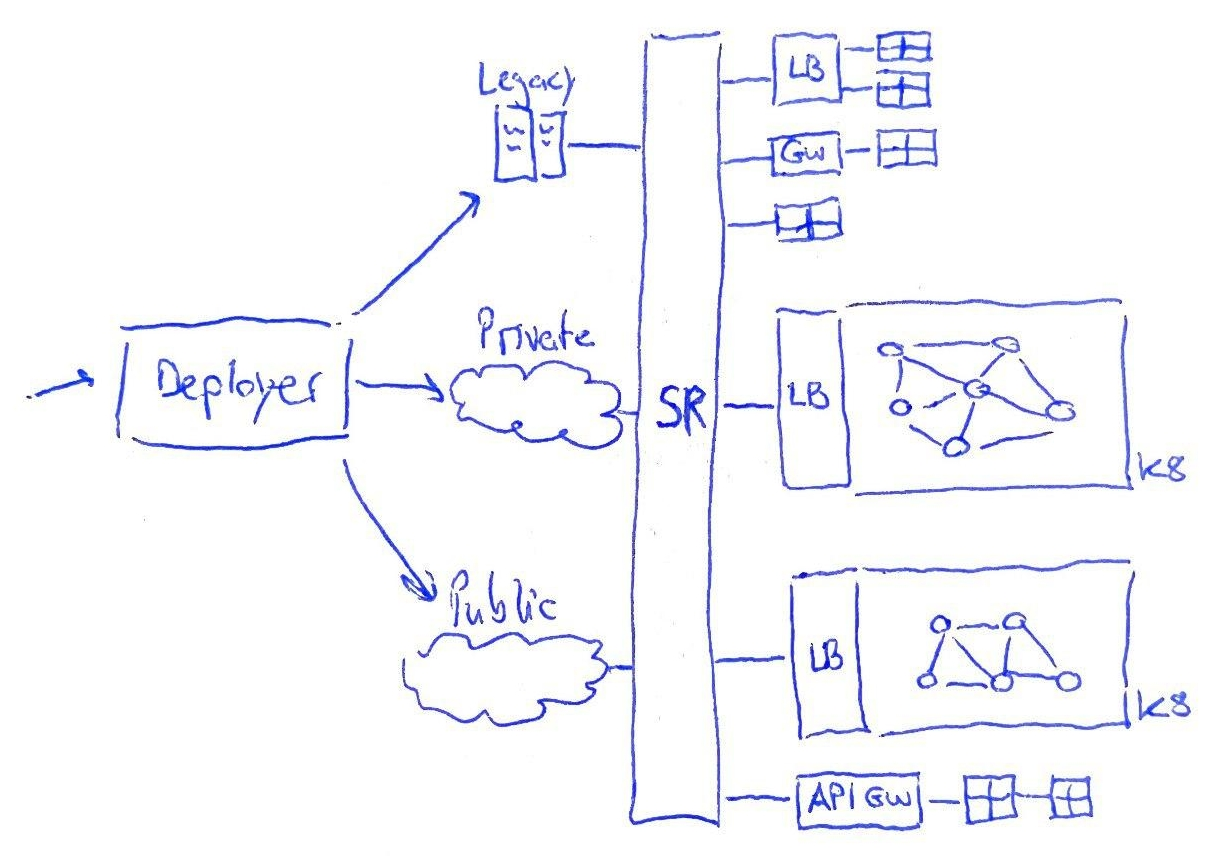
\includegraphics[width=.8\linewidth]{img/abandoned_deploy_registry.jpg}
        \captionsetup{justification=centering}
        \caption{
            A service registry keeps track of all the services deployed and allows the individual components to communicate no matter where they are deployed.
            Requires integration with the service registry.
        }
        \label{fig:deploy_svc_registry}
    \end{figure}

    For computationally heavy processes that also generate a lot of network traffic, resource placement should be reviewed carefully as ingress and egress traffic usually comes with additional cost.
    It might be worth limiting the traffic between on-premise and \gls{public_cloud} applications to a minimum.

\end{document}

